% !TEX root = ../main.tex
\section{Introduction}

\section{Background and Motivation}

\section{Methodology}

\section{Modular Workflow}
The modular workflow for DPMs, detailed in sub-sections \ref{subsec:blockchain_infra} through \ref{subsec:economic_tradeoff} , outlines key components and decision pathways involved in platform development and operation. Initially, designers select an appropriate blockchain infrastructure, evaluating trade-offs between Layer-1 mainnet's decentralization and security versus Layer-2's cost and throughput efficiencies, considering bridging delays and associated security risks (Section~\ref{subsec:blockchain_infra}). Following this, market creation is structured by deciding on permissioned or permissionless market listing models (Section~\ref{subsec:market_setup_init}). Next, the workflow addresses the tokenization of market outcomes (Section~\ref{subsec:market_mechcanics}) and implements suitable trading mechanisms such as automated market makers (AMMs), limit order books, or a hybrid combination of both (Section~\ref{subsec:price_bootstrapping}). After market closure, the platform utilizes either centralized or decentralized oracle systems, including potential dispute resolution processes for contested outcomes (Section~\ref{subsec:market_resolution}). Subsequent stages involve selection of payout methods (automatic push or claim-based pull) and managing remaining funds or platform fees (Sections~\ref{subsec:payout_redemption}). The market metadata archival is preserved on-chain logs or decentralized storage services such as IPFS and Arweave (Section~\ref{subsec:archival}). Finally, economic trade-offs affect the popularity usability and adoption of the market ({Section~\ref{subsec:economic_tradeoff}). This modular workflow is visualized in Figure~\ref{fig:dpm_workflow} below.

\begin{figure}[htbp]
    \centering
    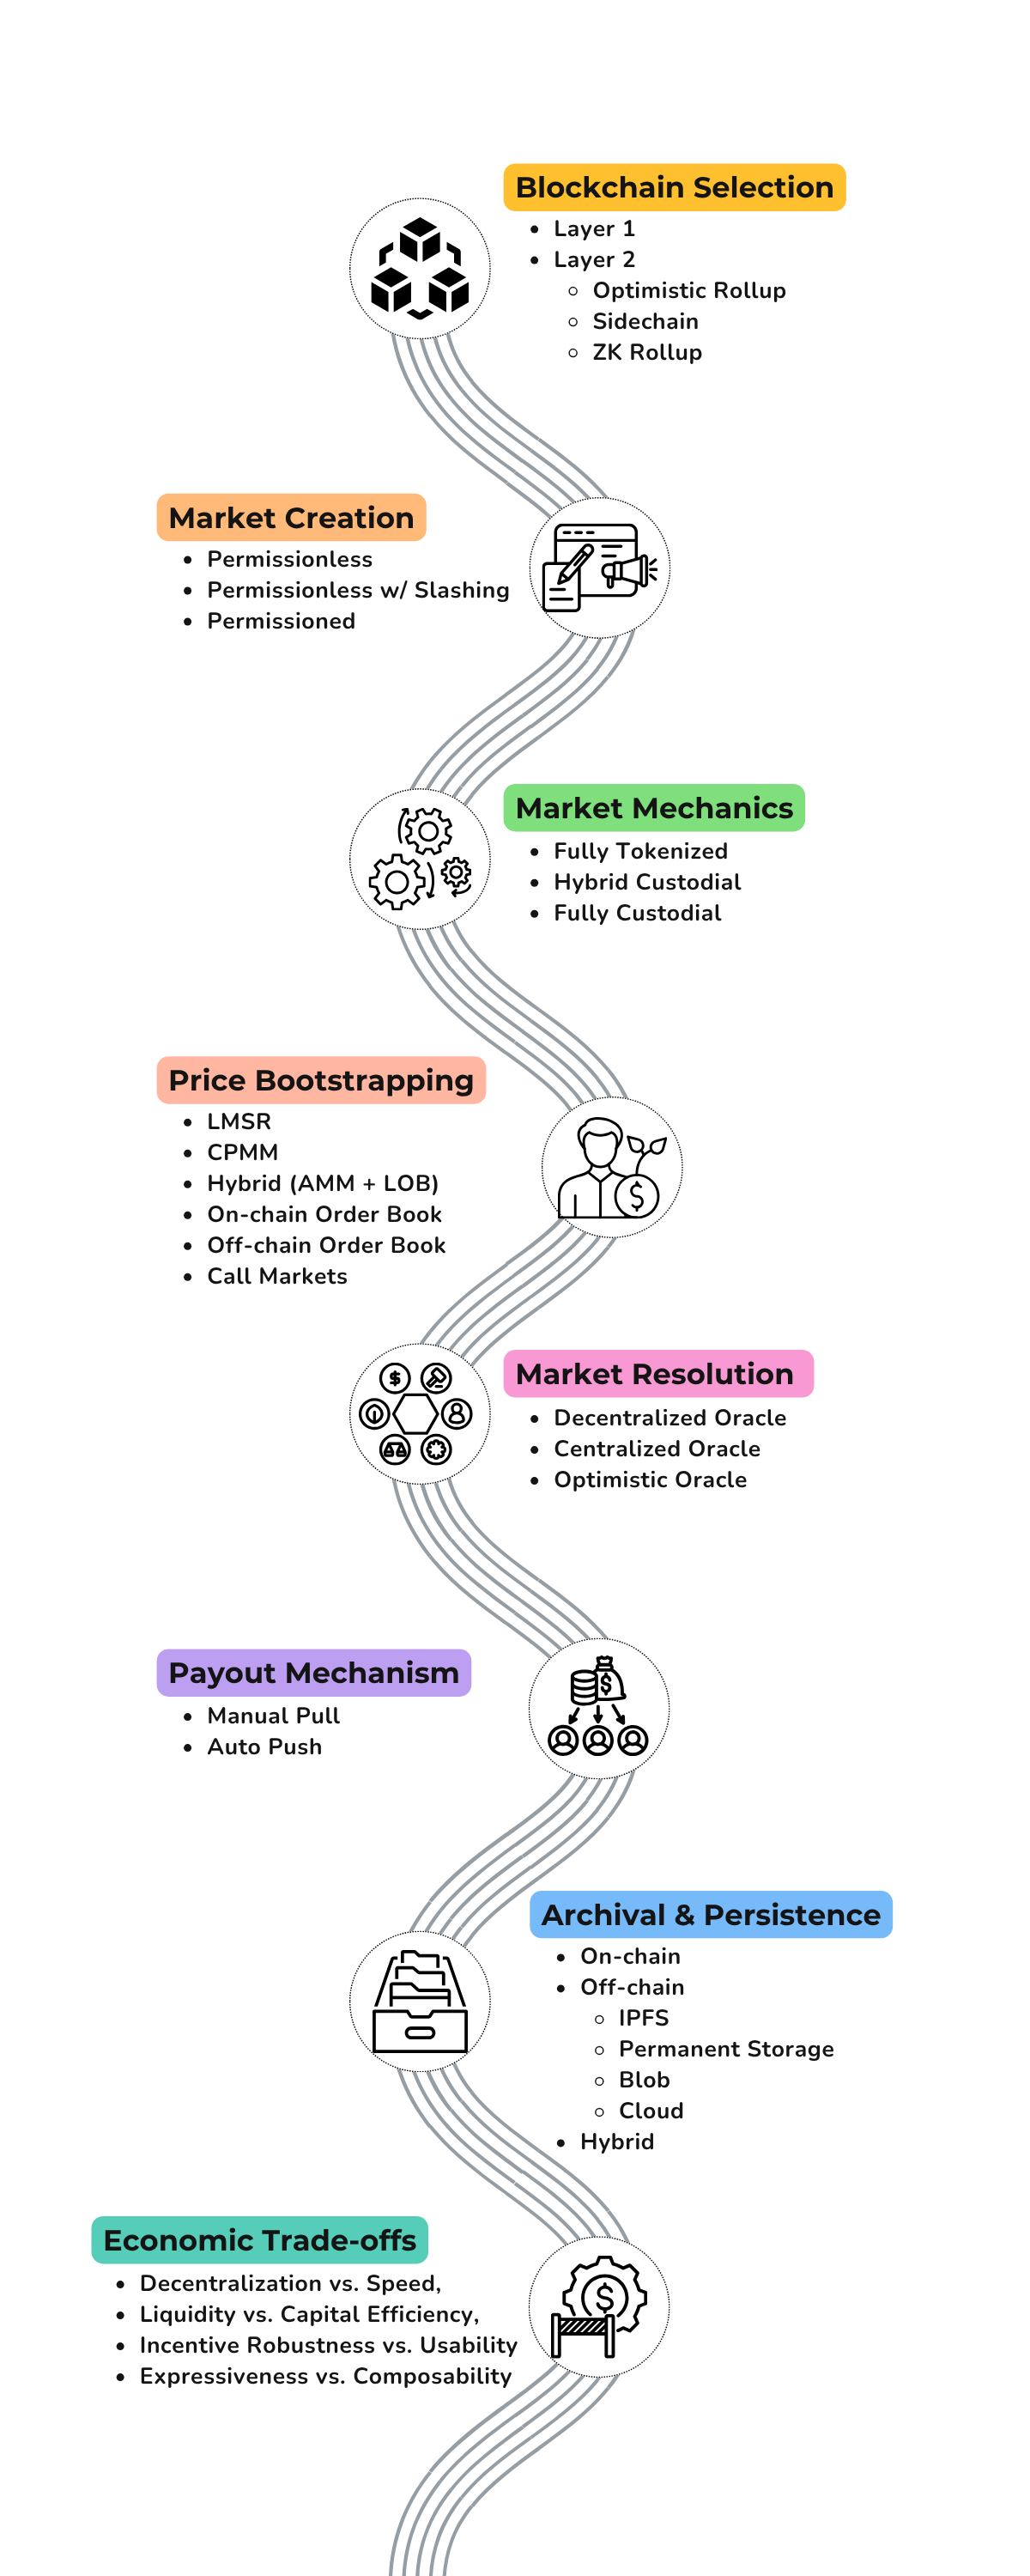
\includegraphics[height=1\textheight]{figures/fig_modular_workflow.png}
    \caption{Modular Workflow for Decentralized Prediction Market Platforms.}
    \label{fig:dpm_workflow}
\end{figure}

\subsection{Underlying Blockchain Infrastructure}\label{subsec:blockchain_infra}
The base blockchain layer (Layer-1 vs. Layer-2) impacts transaction fees, finality guarantees, throughput, and censorship resistance for DPMs, influencing the efficiency and reliability of each stage within the DPM modular workflow. Selecting the underlying blockchain infrastructure constitutes the initial design decision within the modular workflow for DPMs.

Ethereum Layer-1 (L1) mainnet uses proof-of-stake consensus with explicit finality at approximately 13-minute intervals post-Merge, incurring transaction fees typically between \$1 and \$20 and supporting throughput of around 15--30 transactions per second (TPS)~\cite{ClEsGS21}. The relatively higher fees and limited throughput can restrict frequent trading activities and real-time market responsiveness within the DPM modular workflow.

Bitcoin's proof-of-work consensus results in probabilistic finality, generally confirmed after around 60 minutes, with throughput around 7 TPS and fees from \$1 to \$5, impacting the settlement timing and reliability of outcome reporting and payouts in DPMs~\cite{BCFKMN14}. Ethereum's implementation of proposer/builder separation (PBS) and fair-ordering protocols addresses maximal extractable value (MEV) risks, mitigating transaction front-running and block reordering threats that could compromise fairness within market trading and resolution stages~\cite{BBDGJKLZ19}.

Layer-2 (L2) solutions, including optimistic and Zero Knowledge (ZK) rollups, reduce fees to few cents per transaction and improve throughput to thousands of TPS, facilitating high-frequency trading and timely market resolution. Optimistic rollups introduce withdrawal delays of around 7 days due to fraud-proof verification, complicating liquidity management and affecting timely payouts in the market settlement stage. ZK rollups, using validity proofs, offer quicker withdrawal options, beneficial for improving liquidity availability in the workflow~\cite{AKN21}. However, the centralization of sequencers in some L2 platforms like Arbitrum introduces potential censorship issues, partially mitigated by reducing forced-inclusion delays from 24 to 4 hours, thereby influencing market openness and fairness during trading and settlement phases~\cite{BNCD17}.

Bitcoin’s simpler architecture provides resistance to blockchain reorganizations but lacks detailed MEV mitigation, potentially exposing prediction markets to transaction ordering vulnerabilities. Bridging infrastructure connecting L1 and L2 platforms introduces additional latency, complexity, and security risks, potentially disrupting seamless market transitions between layers. Multisig custodians and relay validators involved in bridging have historically been susceptible to financial exploits, highlighting critical risks to asset safety and liquidity flow within the modular workflow of DPMs.

Table \ref{tab:blockchain_infra} below summarizes the performance and decentralization characteristics of blockchain infrastructures relevant to the DPM modular workflow. These infrastructure characteristics shape the feasibility of subsequent market design elements, including market setup and initialization.

\begin{table}[htbp]
    \centering
    \caption{Comparative Attributes of Blockchain Infra for DPM Platforms}
    \begin{tabular}{
        |p{3.2cm}|
        >{\centering\arraybackslash}p{3.2cm}|
        >{\centering\arraybackslash}p{3.2cm}|
        >{\centering\arraybackslash}p{3.2cm}|
     }
         \hline \textbf{Attribute} & \textbf{Ethereum Mainnet} & \textbf{Polygon} & \textbf{Bitcoin} \\
         \hline Transaction Latency & $\sim$12--15 sec/block; \newline $\sim$13 min finality & $\sim$2--5 sec/block & $\sim$10 min/block; \newline $\sim$60 min finality \\
         \hline Bridging Delays & $\sim$7 days \newline (Optimistic Rollups) & $\sim$30 min--3 hrs \newline (Checkpointing) & $\sim$60 min \newline (Sidechains) \\
         \hline Transaction Costs & High \newline (\$1--20+ per tx) & Very low \newline (\$0.01--0.05 per tx) & Moderate-high \newline (\$1--5+ per tx) \\
         \hline Throughput (TPS) & $\sim$15--30 TPS & $\sim$7,000 TPS (peak) & $\sim$7 TPS \\
         \hline Validator Decentralization & High \newline ($\sim$600,000 validators) & Moderate \newline ($\sim$100--150 validators) & High \newline (large miner base) \\
         \hline Censorship Resistance & High \newline (MEV risk present) & Moderate \newline (checkpoint risk) & High \newline (minimal MEV risk) \\
         \hline
    \end{tabular}
    \label{tab:blockchain_infra}
\end{table}

Explicit finality mechanisms, such as Ethereum’s proof-of-stake consensus, provide certainty regarding transaction irreversibility after a specific period, enabling precise timing for market settlements and payouts~\cite{ClEsGS21}. In contrast, probabilistic finality, characteristic of Bitcoin’s proof-of-work, introduces uncertainty, requiring multiple block confirmations, thereby delaying final market outcomes and associated payout distributions~\cite{BCFKMN14}.

\subsection{Market Setup and Initialization}\label{subsec:market_setup_init}
Market setup and initialization choices influence censorship resistance, regulatory compliance, and operational effectiveness of DPMs.

\paragraph{Permissionless Models:} In permissionless setups, such as Augur, any user can initiate markets without centralized oversight, enabling maximum censorship resistance and innovation~\cite{Du19}. This openness creates potential regulatory challenges, illustrated by Augur's "assassination markets" controversy, where third-party moderation efforts (e.g., Predictions.Global) were limited in effectiveness. Economic penalties like validity and no-show reporter bonds address malicious or ambiguous market creation. Permissionless setups typically encourage standardized event templates to minimize ambiguity, though custom markets remain allowed. Collateral selection often involves endogenous (native) tokens (e.g., ETH for Augur), introducing volatility risk and regulatory complexity, balanced by potential hedging benefits when outcomes correlate with token value~\cite{AKPWZ19}~\cite{Sz15}.

\paragraph{Hybrid Governance Models (Permissionless with Centralized Slashing):} Hybrid models allow permissionless market creation combined with centralized oversight mechanisms. Platforms like Polymarket use entities such as a Market Integrity Committee to enforce compliance and penalize markets violating rules~\cite{ClEsGS21} ~\cite{Du19}. This partially decentralizes market listing but maintains centralized control, creating regulatory accountability and single points of control. Hybrid platforms also leverage standardized event templates to maintain clarity and reduce dispute risk, supplemented by custom market oversight. Collateral choices generally include stablecoins, reducing volatility exposure and regulatory uncertainty compared to endogenous tokens.

\paragraph{Permissioned Models:} Fully permissioned setups, including Kalshi and PredictIt, require internal or regulatory reviews before listing markets, significantly reducing regulatory and operational risks by limiting ambiguous or unlawful markets ~\cite{BCFKMN14}. Market proposals typically use standardized event templates to ensure unambiguous resolution, supported by rigorous internal review. Collateral is generally stablecoins or fiat currency, minimizing volatility and simplifying regulatory compliance. Strict implementation of KYC/AML protocols further reduces regulatory exposure, though it introduces operational overhead and restricts market diversity~\cite{Du19}.

Table \ref{tab:market_setup_init} summarizes operational implications for each market setup, guiding stakeholders in selecting appropriate governance models based on desired censorship resistance, compliance requirements, and collateral management.

\begin{table}[htbp]
     \centering
     \caption{Comparative Evaluation of Market Creation and Permission Models}
     \begin{tabular}{
         |p{2.6cm}|
         >{\centering\arraybackslash}p{4.3cm}|
         >{\centering\arraybackslash}p{3.4cm}|
         >{\centering\arraybackslash}p{2.5cm}|
     }
         \hline \textbf{Market Setup} & \textbf{Benefits} & \textbf{Drawbacks} & \textbf{Platforms} \\
         \hline Permissionless & Open participation, censorship resistance, flexible collateral (endogenous tokens) & Regulatory risks, potential misuse, collateral volatility exposure & Augur, PlotX, Gnosis \\
         \hline Permissionless with Slashing & Openness balanced by centralized enforcement, stable collateral (stablecoins) & Centralized oversight, regulatory accountability & Polymarket, UMA\textsuperscript{*} \\
         \hline Permissioned & Compliance, controlled market environment, stable collateral (stablecoins, fiat) & Limited diversity, lower censorship resistance, operational overhead & Kalshi, PredictIt, Stox \\
         \hline
    \end{tabular}
    \label{tab:market_setup_init}
    \vspace{0.5em}
    {\footnotesize\textsuperscript{*}UMA is not a DPM in the traditional sense; it is mentioned here due to its Permissionless with Slashing model usage.}
\end{table}

\subsection{Market Mechanics and Share Custodianship}\label{subsec:market_mechcanics}
Market mechanics and share custodianship directly influence the operational efficiency, liquidity, and decentralization of DPMs.

Binary markets offer intuitive simplicity and consolidated liquidity, facilitating hedging via straightforward YES/NO token pairs, as exemplified by Polymarket’s ERC-1155 tokens redeemable for \$1 upon outcome resolution~\cite{AKPWZ19} ~\cite{IOSG20} This binary structure enables users to hedge risks akin to insurance instruments, although extensive hedging activities by risk-averse participants can temporarily distort prices, potentially diverging from true event probabilities until arbitraged by informed traders~\cite{Ha03}.

In contrast, combinatorial markets, which enable complex bets on interdependent outcomes, significantly enhance theoretical information aggregation by capturing correlations and conditional probabilities but impose exponential computational complexity (\#P-hard for LMSR market makers) and cognitive burdens on users~\cite{CFLPW08}~\cite{CP10}. Thus, combinatorial markets have remained largely experimental, given the difficulty in matching trades efficiently without algorithmic support and substantial fragmentation of liquidity (Pennock \& Sami, 2007).

Markets inherently start with zero traders, necessitating careful liquidity bootstrapping to avoid under-collateralization and price manipulation. Safe market initialization requires at least two traders with opposing views (or one trader matched by an automated market maker) to create balanced, fully collateralized initial positions. This balanced issuance is critical to avoid under-collateralization and ensure meaningful initial price discovery; for instance, Polymarket only mints YES and NO shares simultaneously upon matched buyer-seller orders that sum exactly to \$1 collateral ~\cite{BCFKMN14}. Similarly, Augur mandates traders to initially collateralize all outcomes fully, thus guaranteeing solvent market conditions from inception~\cite{AKPWZ19}.

Custodianship models significantly affect decentralization, regulatory visibility, and systemic trust. Fully tokenized on-chain shares (ERC-20/ERC-1155) maximize decentralization and composability within broader DeFi ecosystems. Conversely, centralized custodial models, though enabling simpler KYC/AML integration, inherently risk censorship and unilateral asset control, undermining core decentralized principles~\cite{Du19}. Polymarket notably adopted more centralized custodianship following regulatory enforcement by the CFTC, underscoring the practical impacts of regulatory pressures on market design~\cite{Ma24}.
Table \ref{tab:market_mechcanics} below summarizes custodianship models, highlighting their implications for composability, decentralization, and systemic trust.

\begin{table}[htbp]
    \centering
     \caption{Comparative Analysis of Custody Models for Outcome Tokenization}
     \begin{tabular}{
         |p{2.7cm}|
         >{\centering\arraybackslash}p{2.5cm}|
         >{\centering\arraybackslash}p{2.8cm}|
         >{\centering\arraybackslash}p{3cm}|
         >{\centering\arraybackslash}p{2cm}|
         >{\centering\arraybackslash}p{2.5cm}|
     }
          \hline \textbf{Custody Model} & \textbf{Composability} & \textbf{Regulatory Visibility} & \textbf{Systemic Trust \& Risk} & \textbf{Decentralization} & \textbf{Examples} \\
          \hline Fully Tokenized (ERC-20 / ERC-1155) & High (DeFi interoperability) & High (public) & Smart-contract reliant & High & Augur, Gnosis \\
          \hline Hybrid Custodial & Moderate & Moderate-high (KYC/AML) & Partial central reliance & Moderate & Polymarket, UMA \\
          \hline Fully Centralized & Low (none) & Low visibility, high control & Centralized, censorship risk & Low & Kalshi, PredictIt \\
          \hline
     \end{tabular}
     \label{tab:market_mechcanics}
\end{table}

\subsection{Price Bootstrapping and Liquidity Mechanisms}\label{subsec:price_bootstrapping}
Price bootstrapping and liquidity provision enable initial price formation and continuous trading in DPMs. Automated Market Makers (AMMs) address the bootstrapping challenge by providing immediate liquidity and initial price setting without requiring initial trading counterparties.
The Logarithmic Market Scoring Rule (LMSR), introduced by~\cite{Ha03}, utilizes a convex cost function:
FORMULA REMOVED
	where b>0 defines liquidity depth~\cite{OPRS13}.
LMSR adjusts instantaneous outcome prices using a softmax function to maintain valid probability distributions. LMSR limits liquidity provider losses to a maximum of \( b \ln{N} \) for a market with N outcomes, providing a known loss boundary~\cite{CP10}.
Selecting the liquidity parameter b presents practical challenges; inappropriate values can result in either excessive price sensitivity or limited market responsiveness~\cite{Ha03}.
Constant Product Market Makers (CPMM), such as those based on the invariant:
\[x \cdot y = k\]

manage liquidity by holding two token reserves, with outcome prices determined by the ratio of these reserves~\cite{AC20}. Arbitrage ensures prices generally sum to a valid probability distribution. However, CPMMs expose liquidity providers to divergence loss (impermanent loss), where large shifts in outcome probabilities leave providers holding primarily the less valuable tokens at resolution~\cite{CDM23}. Unlike LMSR, CPMM does not limit potential losses, thus introducing additional financial risk despite operational simplicity and compatibility with decentralized finance (DeFi) protocols.
Hybrid models integrating AMMs with limit order books (LOBs), as implemented by platforms like Polymarket, combine continuous liquidity provided by AMMs with liquidity precision offered by order books~\cite{ClEsGS21}. These hybrid systems facilitate arbitrage-driven adjustments that stabilize market prices and maintain accurate probability reflections, balancing AMM simplicity with order book responsiveness.

Alternative liquidity mechanisms, including pure on-chain order books and periodic call markets, introduce distinct trade-offs, which are detailed in Table 1. Pure on-chain order books offer precise pricing but encounter issues related to transaction latency and high gas fees, whereas off-chain order books mitigate these problems at the expense of decentralization ~\cite{BCFKMN14}. Call markets aggregate trades at regular intervals to improve liquidity but face latency issues and potential arbitrage vulnerabilities due to delayed execution~\cite{ACES17}.

Table \ref{tab:price_bootstrapping} contrasts liquidity mechanisms used in decentralized prediction markets by evaluating their risk characteristics, price formation methods, and operational attributes. Each mechanism presents unique trade-offs, balancing liquidity provider risks, system complexity, arbitrage vulnerabilities, and operational efficiency.

\begin{table}[htbp]
    \centering
    \caption{Comparative Analysis of Liquidity Mechanisms}
    \begin{tabular}{
        |p{3cm}|
        >{\centering\arraybackslash}p{1.6cm}|
        >{\centering\arraybackslash}p{2.5cm}|
        >{\centering\arraybackslash}p{2cm}|
        >{\centering\arraybackslash}p{2.3cm}|
        >{\centering\arraybackslash}p{2.7cm}|
    }
        \hline \textbf{Liquidity Mechanism} & \textbf{Loss Limitation} & \textbf{Price Formation} & \textbf{Complexity} & \textbf{Arbitrage Exposure} & \textbf{Operational Latency} \\
        \hline LMSR & Yes & Softmax pricing & Moderate & Moderate & Low \\
        \hline CPMM & No & Reserve ratios & Low & High & Low \\
        \hline Hybrid (AMM + LOB) & Partial & Mixed & High & Moderate & Low to Moderate \\
        \hline On-chain Order Book & No & Order matching & High & Moderate & High \\
        \hline Off-chain Order Book & No & Order matching & Moderate & Moderate & Low \\
        \hline Call Markets & No & Batch matching & Moderate & High & Moderate to High \\
        \hline
   \end{tabular}
   \label{tab:price_bootstrapping}
\end{table}

\subsection{Market Resolution and Dispute Models}\label{subsec:market_resolution}
Market resolution and dispute models are essential for accurate and fair settlement in DPMs, directly affecting market credibility and operational continuity.
Single-trusted entity models utilize a single oracle, such as the Associated Press, enabling efficient and rapid finalization. However, reliance on a single entity introduces centralization risks, including vulnerability to bribery and biased reporting~\cite{ClEsGS21}. Economic deterrents like escrow bonds may not prevent manipulation if potential gains surpass the penalties.

Decentralized oracle collectives distribute decision-making across multiple oracles. Chainlink aggregates data from independent nodes using median or majority votes, with nodes required to stake tokens, incentivizing accuracy and penalizing errors. MakerDAO uses governance-based collectives, electing trusted data feeders through community governance to enhance transparency and reduce individual collusion risks~\cite{ClEsGS21}. These collectives, however, experience higher latency and complexity and remain susceptible to coordinated manipulation and governance capture. UMA’s Data Verification Mechanism (DVM) dynamically calculates stakes based on the Cost of Corruption versus Profit from Corruption, aiming to ensure corruption costs always exceed potential profits~\cite{CLL19}. Realitio employs a tiered dispute escalation process, resolving uncontested outcomes swiftly while disputed cases escalate to external arbitrators like Kleros, balancing speed and decentralization.

Self-settling models depend entirely on internal incentives to align reporter behaviour around Schelling points. Augur exemplifies this, with REP tokens staked to encourage reporting consistent with the majority's expectations. Disputes trigger increased staking requirements and potentially protocol forks, reinforcing truthful reporting through economic incentives~\cite{AKPWZ19}. Yet, these mechanisms are vulnerable to coordinated bribery and external manipulation, especially when attackers exploit side-bet strategies~\cite{BF19}. An attacker-defender payoff matrix clearly illustrates these economic vulnerabilities, highlighting equilibrium conditions shaped by manipulation costs and incentives.

Table \ref{tab:market-resolution-types} provides a comparative evaluation of oracle types, outlining operational characteristics, specific risks, and representative examples. It succinctly differentiates between single trusted entities, decentralized oracle collectives, and self-settling oracles by highlighting advantages such as decentralization levels and inherent vulnerabilities like susceptibility to bribery.

\begin{table}[htbp]
    \centering
    \caption{Comparative Evaluation of Market Resolution Types}
    \begin{tabular}{
        |p{3.5cm}|
        >{\centering\arraybackslash}p{3.5cm}|
        >{\centering\arraybackslash}p{3.8cm}|
        >{\centering\arraybackslash}p{3.5cm}|
    }
       \hline \textbf{Oracle Type} & \textbf{Pros} & \textbf{Cons} & \textbf{Examples} \\
       \hline Single Trusted Entity & Fast resolution; clear accountability & Single failure point; high censorship risk & Associated Press, Chainlink \\
       \hline Decentralized Oracle Collective & Distributed trust; censorship resistance & Higher complexity; risk of collusion & UMA, Realitio, MakerDAO \\
       \hline Self-Settling (Schelling-Point) & No external trust; economic incentives & Vulnerable to bribery; fork complexity & Augur, Truthcoin, Kleros \\
       \hline
     \end{tabular}
     \label{tab:market-resolution-types}
\end{table}

Table \ref{tab:oracle-payoff-matrix} presents a detailed incentive compatibility payoff matrix for Augur’s REP staking mechanism. It describes four distinct situations with different combinations of attacker and honest stakes, and potential rewards if an attacker succeeds versus consequences if defenders successfully prevent the attack. The first scenario shows stability when no attack occurs and reporting remains honest, generating standard rewards. In the second scenario, a small attacker stake versus a larger honest stake renders attacks unlikely due to limited attacker profitability. However, in scenarios with higher attacker stakes or significant external bets, the table demonstrates potential attacker profitability, making bribery economically viable and possibly leading to the breakdown of the Schelling point equilibrium.

\begin{table}[htbp]
    \centering
    \caption{Oracle Incentive Compatibility Payoff Matrix (Example: Augur REP Game)}
    \begin{tabular}{
        |p{3.2cm}|
        >{\centering\arraybackslash}p{2cm}|
        >{\centering\arraybackslash}p{1.6cm}|
        >{\centering\arraybackslash}p{2.2cm}|
        >{\centering\arraybackslash}p{2.6cm}|
        >{\centering\arraybackslash}p{3cm}|
    }
        \hline \textbf{Scenario} & \textbf{Attacker Stake (A)} & \textbf{Honest Stake (H)} & \textbf{Attacker Reward if Successful} & \textbf{Defender Reward if Successful} & \textbf{Equilibrium Result} \\
        \hline No Attack, Honest Majority & \$0 & \$1,000,000 & \$0 & \$0 \newline (normal fees) & Honest Reporting Stable \\
        \hline Attack, Low Attacker Stake & \$500,000 & \$1,000,000 & \$10,000,000 & Attacker's stake \newline (slashed) & Honest Reporting Stable \newline (Attack Unlikely) \\
        \hline Attack, High Attacker Stake & \$1,500,000 & \$1,000,000 & \$10,000,000 & Attacker's stake \newline (slashed) & Attacker Profitable \newline (Bribe Possible) \\
        \hline Coordinated Side-Bet Bribery & \$2,000,000 & \$1,000,000 & \$20,000,000 \newline (external bets) & Attacker's stake \newline (slashed) & Attack Profitable \newline (Schelling Point Fails) \\
        \hline 
    \end{tabular}
    \label{tab:oracle-payoff-matrix}
\end{table}



To mitigate vulnerabilities identified in Table 6, designers can implement thresholds for stake escalation and require proportionally larger attacker stakes relative to honest stakes to disrupt equilibrium~\cite{AKPWZ19}. Additionally, periodic audits or community-based moderation processes may deter coordinated attacks, reinforcing equilibrium stability~\cite{ClEsGS21}.

\subsection{Payout and Redemption Mechanisms}\label{subsec:payout_redemption}
DPMs commonly implement push or pull payout mechanisms, each presenting distinct trade-offs. Push payout models automatically distribute winnings once market outcomes are resolved, reducing user interaction requirements. However, they face scalability and cost constraints due to increased gas usage, especially in scenarios involving numerous recipients~\cite{ClEsGS21}. Polymarket uses a hybrid model on the Polygon network with USDC that mimics push mechanisms via meta-transactions, effectively removing direct user gas fee payments~\cite{Ma24} Castle Capital, 2024). Conversely, Augur utilizes a pull mechanism, requiring users to manually redeem tokens to collect payouts. This approach prioritizes decentralization but increases the complexity and cost associated with claiming rewards~\cite{AKPWZ15}.

Gasless redemption mechanisms aim to improve usability by eliminating user gas fees, typically relying on third-party relayers to cover transaction costs. Such mechanisms enhance accessibility but introduce dependencies on centralized components, creating potential points of failure or censorship (Castle Capital, 2024).

Time-bounded redemption windows set deadlines for payout claims, aiming to reduce inefficiencies caused by permanently locked collateral. These mechanisms can enhance capital utilization but raise ethical and regulatory concerns, including issues related to unclaimed property regulations and user fairness~\cite{ClEsGS21}. Major platforms like Augur and Polymarket generally favor open-ended claims to uphold continuous user rights.

Surplus management deals with residual funds from unclaimed or locked winnings. Permanent locking maintains explicit user ownership at the expense of economic efficiency over time, exemplified by Augur’s approach~\cite{ClEsGS21}. Redistribution methods periodically allocate surplus to liquidity providers or active users, increasing capital efficiency but potentially creating incentives to abandon minor balances intentionally. Governance-controlled treasuries allow directed surplus management, balancing efficiency against the risk of centralized governance influence and regulatory attention~\cite{BMR17}.

Table \ref{tab:surplus-management} compares surplus management methods in decentralized prediction markets, evaluating their economic efficiency, ethical considerations, and regulatory implications. It identifies trade-offs between preserving explicit user ownership and maximizing capital efficiency, highlighting potential governance risks and compliance requirements for different mechanisms.

\begin{table}[htbp]
    \centering
    \caption{Comparative Evaluation of Surplus Management Mechanisms}
    \begin{tabular}{
        |p{2.5cm}|p{3.8cm}|
        >{\centering\arraybackslash}p{2cm}|
        >{\centering\arraybackslash}p{2.5cm}|
        >{\centering\arraybackslash}p{2.5cm}|
        >{\centering\arraybackslash}p{2.5cm}|
    }
        \hline \textbf{Mechanism} & \textbf{Description} & \textbf{Economic Efficiency} & \textbf{Ethical Considerations} & \textbf{Regulatory Implications} & \textbf{Example Platforms} \\
        \hline Permanent Locking & Surplus funds locked indefinitely post-resolution & Low & Maintains explicit user ownership & Low regulatory risk & Augur, Gnosis \\
        \hline Redistribution to LPs/Stakers & Surplus periodically redistributed to liquidity providers & High & May incentivize intentional abandonment & Moderate, potential property concerns & UMA, Realitio \\
        \hline Governance-controlled Treasury & Surplus directed by governance structures & Moderate–High & Potential governance influence risk & Moderate–High, regulatory attention & Polymarket, SX Network \\
        \hline Burning Tokens & Surplus tokens destroyed to reduce supply & Moderate–High & Minimal ethical concerns & Moderate, regulatory stance uncertain & Truthcoin (theoretical) \\
        \hline Returning to Original Funders & Surplus returned to initial market creators & Moderate & Risks manipulation incentives & High, KYC and AML compliance concerns & Kalshi \\
        \hline
    \end{tabular}
    \label{tab:surplus-management}
\end{table}

\subsection{Archival, Transparency, and Meta-Data Persistence}\label{subsec:archival}
Archival, transparency, and metadata persistence within DPMs ensure verifiable and accessible records, directly impacting market integrity and governance processes.

Critical metadata, such as market states, transaction histories, and resolution outcomes, inherently benefit from blockchain immutability and cryptographic verification~\cite{Du19},~\cite{ClEsGS21}. Augur v2 stores metadata, including user profit/loss computations, directly on-chain, providing immediate access without external archives. This design increases transparency but also results in higher transaction costs and larger blockchain state size~\cite{Fo20}.

Off-chain metadata - including market descriptions, resolution criteria, and user-generated content - are typically stored in decentralized storage solutions due to blockchain capacity constraints~\cite{BCCJM21}. IPFS (InterPlanetary File System) employs peer-to-peer, content-addressable storage using cryptographic hashes, verifying content authenticity through immutable identifiers. IPFS’s availability depends on node operators maintaining persistent storage through pinning, without central points of failure~\cite{IM24}. Arweave offers an economic incentive structure combined with a "blockweave" architecture for permanent data storage, providing perpetual availability and resistance to censorship~\cite{BCKW23}.

Recent updates to Ethereum, such as proto-danksharding, provide ephemeral "blob" storage. These storage blobs temporarily allow for large metadata availability and cryptographic verification. However, their short-term nature necessitates subsequent migration to persistent storage solutions~\cite{Fo20}.

The archival model chosen by a DPM influences governance outcomes and resilience against manipulation. Persistent archival supports retrospective audits critical for resolving disputes and maintaining accountability of oracle activities~\cite{ClEsGS21}. Decentralized archival mechanisms prevent centralized control from suppressing or altering market data, enabling community-driven governance or protocol forks when required~\cite{BCKW23}.

Table \ref{tab:archival-methods} compares archival methods such as blockchain storage, IPFS, Arweave, Ethereum blob storage, and hybrid models. It details each method's durability, authenticity, and accessibility, highlighting their distinct operational trade-offs and cost implications for decentralized prediction markets.

\begin{table}[htbp]
    \centering
    \caption{Comparative Evaluation of Archival Methods for Decentralized Prediction Markets}
    \renewcommand{\arraystretch}{1.3}
    \begin{tabular}{
        |p{2.3cm}|
        p{3cm}|
        >{\centering\arraybackslash}p{2.0cm}|
        >{\centering\arraybackslash}p{2.5cm}|
        >{\centering\arraybackslash}p{2.8cm}|
        >{\centering\arraybackslash}p{2.6cm}|
    }
        \hline \textbf{Archival Method} & \textbf{Description} & \textbf{Durability \& Persistence} & \textbf{Authenticity \& Integrity} & \textbf{Accessibility \& Discovery} & \textbf{Example Platforms} \\
        \hline Blockchain On-chain Storage & Directly store metadata and outcomes on-chain (e.g., Ethereum). & Extremely high (immutable, perpetual) & High authenticity (cryptographic guarantees) & Excellent (immediate, global nodes) & Augur (partial), Gnosis \\
        \hline IPFS (InterPlanetary File System) & Decentralized, peer-to-peer, content-addressable storage. & Medium (requires community pinning) & High (content hashes provide tamper-evidence) & Good (distributed nodes, variable retrieval speeds) & Augur, Polymarket \\
        \hline Arweave Permanent Storage & Blockchain-based storage with economic incentives for permanent retention. & Very high (economically incentivized permanence) & Very high (blockchain-backed immutability) & High (permanent, redundant node distribution) & Mirror.xyz, RedStone Oracles (experimental) \\
        \hline Ethereum Blob Storage & Temporary large-data storage via Ethereum blobs (proto-danksharding). & Low (temporary, ephemeral data availability) & High (cryptographic authenticity guaranteed short-term) & Moderate (short-term retrieval from Ethereum nodes) & Ethereum L2s (Optimism, Arbitrum) \\
        \hline Centralized Cloud Storage & Traditional cloud services (AWS, Google Cloud). & Variable (single point of failure risk) & Low–moderate (trust reliant on centralized operator) & High (fast retrieval, easy indexing) & Early centralized prediction platforms \\
        \hline Hybrid Storage Model & Combination: blockchain on-chain pointers plus decentralized or permanent storage. & High (leverages strengths of multiple methods) & High (on-chain hashes guarantee authenticity) & Very high (multiple redundancy points, robust discovery) & Polymarket, UMA \\
        \hline
    \end{tabular}
    \label{tab:archival-methods}
\end{table}

\subsection{Economic Trade-Offs in DPM Design}\label{subsec:economic_tradeoff}
The design of DPMs involves inherent economic trade-offs affecting platform adoption, integrity, and resilience. This analysis examines these trade-offs across four dimensions: decentralization versus speed, liquidity versus capital efficiency, incentive robustness versus usability, and expressiveness versus composability, with agility noted as an additional consideration.

A fundamental trade-off occurs between decentralization and execution speed. Fully decentralized DPMs, such as early Augur versions, achieve censorship resistance but experience latency and high transaction costs due to reliance on Ethereum’s mainnet~\cite{BCFKMN14}~\cite{AKPWZ15}. Hybrid models, including Polymarket, employ off-chain order matching and on-chain settlements or dedicated sidechains to increase throughput and improve usability, albeit with the addition of trust assumptions and centralization risks~\cite{ClEsGS21}. Layer-2 technologies like state channels and rollups offer alternative methods to balance decentralization and performance~\cite{BBMMM19}.

Liquidity provision versus capital efficiency presents another critical trade-off. Automated market makers (AMMs), such as Hansonian market scoring rules or constant product market makers (CPMM), deliver continuous liquidity by committing substantial collateral, reducing capital efficiency~\cite{Ha03}~\cite{AC20}. Conversely, order-book-based models maximize capital efficiency by avoiding idle capital but can encounter liquidity issues and impaired price discovery, as noted in Augur v1 markets~\cite{AA20}. Platforms like Gnosis address some of these challenges through conditional markets that dynamically allocate capital among outcomes~\cite{Gn17}.

Incentive robustness and usability reflect another key trade-off. Augur’s multi-stage dispute mechanisms and token staking enhance manipulation resistance but complicate user experience and slow resolution processes~\cite{AKPWZ15}~\cite{ClEsGS21}. In contrast, simplified oracle solutions, such as UMA's optimistic oracle, offer streamlined resolution processes but carry greater risks of manipulation. Hierarchical or two-tiered dispute frameworks (e.g., Pisa watchtowers) seek to address these issues by maintaining manipulation resistance while minimizing complexity~\cite{BBMMM19}.

Expressiveness versus composability represents an additional design dimension. Highly expressive combinatorial market structures, such as those enabled by Gnosis’s Conditional Tokens, allow detailed market configurations but reduce interoperability and composability with other decentralized finance (DeFi) systems due to technical complexity~\cite{Gn17}. Simpler binary or categorical markets increase interoperability and composability but sacrifice detailed market structuring capabilities.


\section{Security and Adversarial Considerations}

\section{Regulatory and Ethical Considerations}

\section{Case Studies}

\section{Future Directions and Open Challenges}

\section{Conclusion} 
% = = = = = = = = = = = = = = = = = = = = = = = = = = = = = = = = = = = = = = = = = =

\paragraph{Scope.} 
Blah blah blah.

% = = = = = = = = = = = = = = = = = = = = = = = = = = = = = = = = = = = = = = = = = =

\paragraph{Contributions.} 
Our primary contributions are as follows.

\begin{enumerate}

\item Blah blah blah.

\item Blah blah blah. 

\item Blah blah blah. 

\end{enumerate}
